\ifx\ISMAIN\undefined
    \documentclass{AsignaturaResumen}
    \usepackage{etoc}
    \SetTitulo{Fenómenos de transporte}
    \setabbreviationstyle[acronym]{long-short}
\makeglossaries

    % Glosario

\newglossaryentry{latex}{
    name={latex},
    description={Procesador de textos}
}

    % Acrónimos

\newacronym{adn}{ADN}{Ácido desoxirribonucléico}
\newacronym{si}{SI}{Sistema Internacional}
\newacronym{ros}{ROS}{especies reactivas de oxígeno}
\newacronym{iubmb}{IUBMB}{Unión Internacional de Bioquímica y Biología Molecular}
\newacronym{pcr}{PCR}{Reacción en cadena de la polimerasa}
    \begin{document}
    \dominitoc
    \faketableofcontents
    \chapter{Mecanismos de transporte}
    \mymtc
\fi

\section{Presión}\label{sec:presion}

Si se requiere calcular la cantidad de kg totales de un fluido se utiliza:

\begin{equation*}
    kg_{\text{Total}} = h_{2}(m) \cdot A(m^{2}) \cdot \rho(kg/m^{2}) = h_{2} \cdot A \cdot \rho_{g} 
\end{equation*}

Para calcular la fuerza total ($F$) del fluido sobre el área 1 debido unicamente al fluido es:

\begin{equation}
    F = (h_{2} \cdot A \cdot P)(g)
\end{equation}

\begin{equation}
    P = \frac{F}{A} \quad\therefore\quad P = h_{2} \cdot \rho_{g}
\end{equation}

Esta es la presión sobre A\sub{2} debido a la masa del fluido que está encima. Sin embargo, para obtener la presión total (P\sub{2}) sobre A\sub{2}debe añadirse P\sub{0}, que soporta todo el líquido, de tal manera que:

\begin{equation}
    F = h_{2} \cdot \rho_{g} + P_{0}
\end{equation}

Esta ecuación es la expresión fundamental para calcular la presión de un fluido a cualquier profundidad.

Para P\sub{1}:

\begin{equation}
    P_{1} = h_{1} \cdot \rho_{g} + P_{0}
\end{equation}

La diferencia entre los dos puntos es:

\begin{equation}
    P_{2} - P_{1} = (h_{2} \cdot \rho_{g} + P_{0}) - (h_{1} \cdot \rho_{g} + P_{0})
\end{equation}

\marginpar{\begin{minipage}{\marginparwidth}
    \begin{figure}[H]
        \centering
        \resizebox{\linewidth}{!}{\begin{tikzpicture}[
    principal/.style={line width=1pt},
    trasera/.style={dashed, line width=1pt},
    flecha/.style={|-Stealth},
    delimitador/.style={|-|, line width=0.75pt},
    texto/.style={font=\sffamily}
]

\draw[principal] (2.5,-2.5) -- (-2.5,-2.5) -- node[pos=0.4] (esq4) {} (-2.5,2.5) -- (2.5,2.5) -- node[pos=0.6] (esq3) {} (2.5,-2.5);
\draw[principal] (-5,0) -- node[pos=0.4] (esq1) {} (-5,5) -- (0,5);
\draw[principal] (-5,5) -- (-2.5,2.5);
\draw[principal] (-5,0) -- (-2.5,-2.5);
\draw[principal] (2.5,2.5) -- (0,5);

\draw[trasera] (0,5) -- node[pos=0.6] (esq2) {} (0,0) -- (-5,0);
\draw[trasera] (0,0) -- (2.5,-2.5);

\draw[trasera] (esq1) -- (esq2) -- (esq3) -- (esq4) -- (esq1);

\draw[delimitador] (3.5,2.5) -- (3.5,0) node[midway, left=0pt, texto] {h$_{1}$};
\draw[delimitador] (3.5,0) -- (3.5,-2.5) node[midway, left=0pt, texto] {h$_{3}$};
\draw[delimitador] (4.5,2.5) -- (4.5,-2.5) node[midway, left=0pt, texto] {h$_{2}$};


\draw[flecha] (-6,4) node[texto, left=0pt] {A$_{0}$} -- (-3.25,4);
\draw[flecha] (-6,1.25) node[texto, left=0pt] {A$_{1}$} -- (-3.25,1.25);
\draw[flecha] (-6,-0.75) node[texto, left=0pt] {A$_{2}$} -- (-3.25,-0.75);

\draw[flecha] (-0.8,6) -- (-0.8,3.75) node[texto, pos=0.8, right=0pt] {P$_{0}$};
\draw[flecha] (-0.8,3.5) -- (-0.8,0.5) node[texto, pos=0.8, right=0pt] {P$_{1}$};
\draw[flecha] (-0.8,0.25) -- (-0.8,-1.75) node[texto, pos=0.7, right=0pt] {P$_{2}$};
\end{tikzpicture}}
        \rule{\linewidth}{0.5pt}
        \caption{Ejemplo para representar las diferentes alturas tomadas en cuenta para las ecuaciones presentadas.}
    \end{figure}
\end{minipage}}

\resumebox{ejercicio}{Calculo de presión}{\footnotesize
    Un gran tanque de almacenamiento contiene petroleo de una densidad igual a \qty{917}{\kg\per\m\cubed}. El tanque tiene una altura de \qty{3.66}{\m} y está abierto a la atmósfera con una presión de 1atm absoluta en la superficie. El tanque está lleno con petroleo a una profundidad de \qty{3.05}{\m} y contiene tambien \qty{0.61}{\m} de agua en la parte inferior. calcule la presión en pascales a \qty{3.05}{\m} de la superficie y en el fondo del tanque. También calcule la presión manométrica del fondo del tanque.
}

Los 3 procesos de transporte molecular se caracterizan por el mismo tipo general de ecuación de transporte:

\begin{equation}
    \text{Velocidad de transporte molecular} = \frac{\text{Fuerza impulsora}}{\text{Resistencia}}
\end{equation}

Esto también se puede expresar como:

\begin{equation}\label{eq:ecuacion_de_transporte_molecular_diferencial}
    \Psi_{z} = \sigma\frac{\mathrm{d}\Gamma}{\mathrm{d}Z}
\end{equation}

Donde:

\begin{itemize}
    \item $\Psi_{z}$ es el flujo de propiedad, es decir, la cantidad de la propiedad que se transfiere por unidad de tiempo a través de una sección transversal unitaria perpendicular a la dirección del fljo en cantidad de propiedad dobre metro cuadrado.
    \item $\sigma$ es la difusividad en metro cuadrado sobre segundo (\uni{\m\squared\per\s}). Indica el gradiente y la resistencia
    \begin{itemize}
        \item La difusividad necesita de un gradiente para ocurrir.
    \end{itemize}
    \item $\Gamma$ es la concentración de la propiedad en cantidad de propiedad sobre metros cúbicos (\unit{\substance\per\m\cubed}). Indica la diferencia entre cantidad de transporte
    \item $Z$ es la distancia de la dirección del flujo en metros.
\end{itemize}

Si el proceso ocurre en un estado estacionario el flujo $\Psi_{z}$ es constante:

\begin{equation*}
    \Psi_{z} \ \mathrm{d}Z = - \sigma \ \mathrm{d}\Gamma
\end{equation*}

Esta es una ecuación diferencial que al resolverla por variables separables nos da:

\begin{equation}
    \Psi_{z} = \frac{-\sigma \ (\Gamma_{2} - \Gamma_{1})}{Z_{2} - Z_{1}}
\end{equation}


\resumebox{ejercicio}{Cálculo de flujo}{\footnotesize
    Se está transportando una propiedad por difusión a través de un fluido en estado estacionario. En un punto 1 determinado, la concentración es de \num{1.37d-2} cantidad de propiedad por metro cuadrado (\unit{\meter\squared}), y \num{0.72d-2} en el punto 2, a una distancia de \qty{0.4}{\m}. La difusividad es de \qty{0.013}{\m\squared\per\s}, y el área de corte transversal es constante.
    \begin{enumerate}
        \item Calcula el flujo
        \item Deduce la ecuación para $\Gamma$ como función de la distancia
        \item Calcule $\Gamma$ en el punto medio de la trayectoria
    \end{enumerate}
}

Al calcular las velocidades de transporte en un sistema usando la ecuación de transporte molecular (\autoref{eq:ecuacion_de_transporte_molecular_diferencial}) es necesario tomar en cuenta la cantidad de esta propiedad que se transporta en todo el sistema. Esto se hace escribiendo una ecuación general de balance o conservación para la propiedad en estado no estacionario.

\begin{align*}
    \text{Tasa de la propiedad que entra} \ &+ \ \text{Tasa de generación de la propiedad}
    \\
    &=
    \\
    \text{Tasa de la propiedad que sale} \ &+ \ \text{Tasa de acumulación de la propiedad}
\end{align*}

La velocidad de entrada es $\Psi_{Z / (Z \cdot 1)}$ en cantidad de propiedad sobre segundo (\unit{\substance\per\s}), mientras que la velocidad de salida es $(\Psi_{Z/Z} + \Delta Z) \cdot 1$ en cantidad de propiedad sobre segundo , donde el área de corte transversal es de \qty{1}{\m\squared}. La velocidad de generación de la propiedad se escribe como $R_{\Delta Z \cdot 1}$, que se mide en cantidad de propiedad sobre segundo por metro cúbico (\unit{\substance\per\m\cubed\per\s}). El término para la acumulación es:

\begin{equation}
    \text{Velocidad de acumulación de propiedad} = \frac{\mathrm{d}\Gamma (\Delta Z \cdot 1)}{\mathrm{d}t} 
\end{equation}

En la cual, si sustituimos, tendríamos:

\begin{equation}
    \Psi_{Z / (Z \cdot 1)} + R_{\Delta Z \cdot 1} = (\Psi_{Z/Z} + \Delta Z) \cdot 1 + \frac{\mathrm{d}\Gamma}{\mathrm{d}t} (\Delta Z \cdot 1)
\end{equation}

\section{Tipos de transporte}

\subsection{Transporte de momento lineal y la ley de Newton}

%\marginpar{\resumebox{definicion}{Primera Ley de Newton}{\footnotesize
%    La primera ley de Newton, o ley de la inercia, establece que un objeto en reposo o en movimiento constante mantendrá ese estado a menos que una fuerza externa neta actúe sobre él.
%}}

Cuandoo un fluido fluye en la dirección X en forma paralela a una superficie sólida existe un gradiente de velocidad dondel a velocidad $V_{x}$ en la dirección X disminuye al acercarse a la superficie en la dirección z. El fluido tiene un momento lineal en dirección X y su concentración es $V_{x}\rho$ (momento lineal sobre metro cúbico), donde el momento lineal tiene unidades de kilogramos por metro sobre segundo (\unit{\kg\m\per\s}). Debido a la difusión aleatoria de las moléculas existe un intercambio de moléculas en la dirección z, moviendose igual número de ellas en cada dirección entre la capa de la molécula que se mueve más rápido y la capa adyacente más lenta. La ley que describe lo anterior es la ley de Newton de la viscosidad para una densidad constante:

\begin{equation}
    \tau_{zx} = \frac{-V \cdot \mathrm{d}(V_{x} \cdot \rho)}{\mathrm{d}z}
\end{equation}

Donde:

\begin{itemize}
    \item $\tau_{zx}$ es el flujo de momento lineal con dirección X en la dirección Z (\unit{\kg\m\per\s})
    \item $V$ es $\frac{\mu}{\rho}$, que representa la difusividad de momento lineal en metro cuadrado por segundo (\unit{\m\squared\per\s})
    \item $z$ es la dirección de transporte o difusión en metros (\unit{\m})
    \item $\rho$ es la densidad en kilogramos por metro cúbico (\unit{\kg\per\m\cubed})
    \item $\mu$ es la viscosodad en kilogramos por metro por segundo (\unit{\kg\per\m\s})
\end{itemize}

\subsection{Transporte de calor y la ley de Fourier}

La ley de Fourier para el transporte molecular de calor o la conducción de calor en un fluido o sólido puede escribirse para una densidad constante y capacidad calorífica (cp) de la siguiente manera:

\begin{equation}
    \frac{qz}{A} = \frac{-\alpha \cdot \mathrm{d}\rho \cdot \unit{\cp} \cdot T}{dz}
\end{equation}

Donde:

\begin{itemize}
    \item $\frac{qz}{A}$ es el flujo de calor en \unit{\joule\per\m\squared\s}
    \item $\alpha$ es la difusividad térmica en \unit{\m\squared\per\s}
    \item $\rho \cdot \unit{\cp} \cdot T$ es la concentración de calor o energía térmica en \unit{\joule\per\m\cubed}
\end{itemize}

Cuando hay un gradiente de temperatura en un fluido se difunden igual número de moléculas entre la región caliente y la más fría.

\subsection{Transporte de masa y ley de Fick}

La ley de Fick para el transporte molecular de masa en un fluido o en un sólido para la concentración total constante del fluido es:

\begin{equation}
    J_{AZ} = -D_{AB} \cdot \frac{\mathrm{d}C_{A}}{\mathrm{d}Z}
\end{equation}

Donde:

\begin{itemize}
    \item $J_{AZ}$ es el flujo de A en kgmol de A sobre \unit{\m\squared\s}
    \item $D_{AB}$ es la difusividad molecular de las moléculas A y B en \unit{\m\squared\per\s}
    \item $C_{A}$ es la concentración de A en \unit{\kg\mole} de A sobre \unit{\m\cubed} (\unit{\kg\mole\per\m\cubed})
\end{itemize}

Donde existe un gradiente de concentración en un fluido se difundirán igual número de moléculas en todas las direcciones de alta y baja concentración, y ocurrirá un flujo neto de masa.

\bigskip

Estos 3 transportes son descritos en estado estacionario, y se puede notar en los 3 términos comunes.


\section{Viscosidad} % Ley de Newton y viscosidad

Cuando un fluido se transporta a través de un canal cerrado se presentan dos tipos de flujo dependiendo de dicho fluido:

\begin{enumerate}
    \item A \emph{velocidades bajas} el fluido tiende a transportarse sin mezclado lateral, y las capas adyacentes se resbalan unas sobre las otras. En este caso no hay corrientes cruzadas perpendiculares a la dirección del flujo, ni tampoco remolinos de fluidos. A este tipo de flujo se le llama \emph{flujo laminar}.
    \item A \emph{velocidades altas} se forman remolinos, lo que conduce a un mezclado lateral. A este tipo de flujo se le llama \emph{flujo turbulento}.
\end{enumerate}

La viscosidad es una propiedad de un fluido que da lugar a fuerzas que se oponen al movimiento relativo de capas adyacentes en el fluido. Para muchos fluidos se ha determinado de forma experimental que la fuerza (F) en Newtons es directamente proporcional a la velocidad $\Delta V_{z}$ en metros sobre segundo (\unit{\m\per\s}). El área en metros cuadrados (\unit{\m\squared}) de la placa usada es inversamente proporcional a la distancia $\Delta y$ en metros (\unit{\m}). Expresada con la ley de viscosidad de Newton, cuando el flujo es laminar:

\begin{equation}
    \frac{F}{A} = -\mu \frac{\Delta V_{z}}{\Delta y}
\end{equation}

Donde $\mu$ es la constante de proporcionalidad llamada viscosidad del fluido en pascales por segundo (\unit{\pascal\s}) o \unit{\kg\per\m\s}. Cuando $\Delta y$ tiende a 0:

\begin{equation}
    \tau_{yz} = -\mu \cdot \frac{dV_{z}}{dy}
\end{equation}

\begin{equation}\footnote{lbf/ft\super{2}}
    \tau_{yz} \ gc = -\mu \cdot \frac{dV_{z}}{dy}
\end{equation}

Las unidades en el \emph{sistema cgs} son \unit{\g\per\s\m}, llamados Poise (P) o Centipoise (cp). 

\resumebox{ejercicio}{Cálculo de esfuerzo cortante}{\footnotesize
    La distancia entre las dos placas es de \qty{0.5}{\cm}. La velocidad de flujo que pasa a través es de \qty{10}{\cm\s}, y el fluido que atraviesa se trata de alcohol etílico a \qty{273}{\K}, cuya viscosidad es de \qty{1.77}{cp}.
    \begin{enumerate}
        \item Calcule el esfuerzo cortante $\tau_{yz}$ y el gradiente de velocidad
        \item Repita en SI
    \end{enumerate}
}

\section{Fluidos newtonianos y no newtonianos}

\marginpar{\begin{minipage}{\marginparwidth}
\begin{figure}[H]
    \centering
    \resizebox{\linewidth}{!}{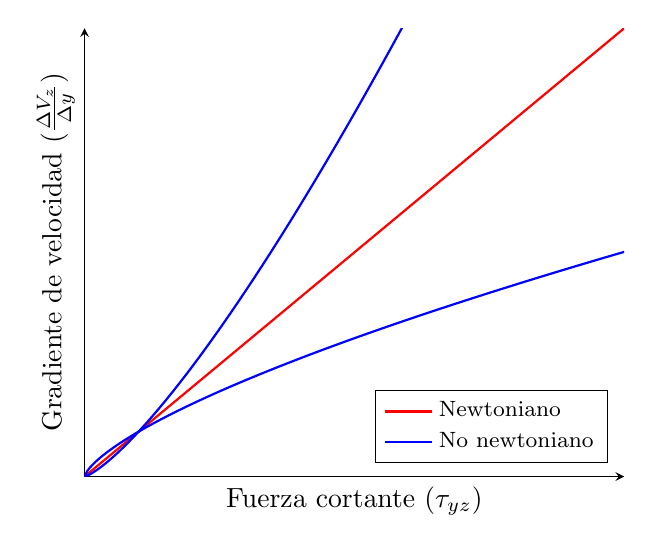
\begin{tikzpicture}
\begin{axis}[
    axis lines = left,
    ticks = none,
    xmin=0, xmax=10,
    ymin=0, ymax=10,
    xlabel = {Fuerza cortante ($\tau_{yz}$)},
    ylabel = {Gradiente de velocidad ($\frac{\Delta V_{z}}{\Delta y}$)},
    domain=0:10, 
    samples=200,
    legend pos = south east,
    legend cell align = left
]
    \addplot[thick, color=red]{x};
    \addlegendentry{\footnotesize Newtoniano}
    \addplot[thick, color=blue]{x^0.7};
    \addplot[thick, color=blue]{x^1.3};
    \addlegendentry{\footnotesize No newtoniano}
\end{axis}
\end{tikzpicture}}
    \rule{\linewidth}{0.5pt}
    \caption{Diferencia entre fluidos newtonianos y no newtonianos}
    \label{fig:grafica_de_tipos_de_fluidos}
\end{figure}
\end{minipage}}

Los fluidos que obedecen la ley de viscosidad e Newton se les llama fluidos newtonianos. En dichos fluidos existe una relación lineal entre el esfuerzo cortante ($\tau_{yz}$) y el gradiente de velocidad ($\frac{\Delta V_{z}}{\Delta y}$), lo cual significa que la velocidad $\mu$ es constante e independiente de la velocidad cortante. En fluidos no newtonianos, la relación entre $\tau_{yz}$ y $\frac{\Delta V_{z}}{\Delta y}$ no es lineal, es decir, $\mu$ no permanece constante, sino que está en función de $\tau_{yz}$.

La viscosidad de los gases, que son fluidos newtonianos, aumenta con la temperatura e independiente de la presión.

\section{Tipos de flujo}

El primer tipo de flujo ocurre a velocidades bajas, donde la capa del fluido parece desplazarse unas sobre las otras sin remolinos o turbulencias. Tal flujo se llama flujo laminar, y obedece la ley de la viscosidad de Newton.

El segundo tipo de flujo ocurre avelocidades más altas, donde se forman remolinos que imparten al fluido una naturaleza fluctante. Este fluido recibe el nombre de flujo turbulento. 

\section{Número de Reynolds (N\sub{Re})}

La expresión para estimar el número de Reynolds es:

\begin{equation}\mathrm{
    N_{Re} = \frac{D \cdot V \cdot \rho}{\mu}
}\end{equation}

Aquí D es el diametro de la tubería en metros (\unit{\m}). V es la velocidad promedio del fondo en metros por segundo (\unit{\m\per\s}), y se obtiene con la velocidad volumétrica del fluida dividida entre el área de corte transversal de la tubería.

Cuando N\sub{Re} es menor a 2100 para una tubería circular recta, el flujo siempre es laminar. Cuand el valor supera 4000 el flujo será turbulento. Entre estos dos valores está la \emph{región de transición}, en la cual el flujo puede ser laminar o turbulento dependiendo de detalles del sistema que no se pueden predecir.

\begin{align*}
    \mathrm{N_{Re}} < 2100        &\quad\longrightarrow\quad \text{Flujo laminar}
    \\
    2100 < \mathrm{N_{Re}} < 4000 &\quad\longrightarrow\quad \text{Región de transición}
    \\
    \mathrm{N_{Re}} > 4000        &\quad\longrightarrow\quad \text{Flujo turbulento}
\end{align*}

\marginpar{\resumebox{ejercicio}{Número de Reynolds}{\footnotesize
    Por una tubería con un diámetro interior de \qty{2.007}{\in} fluye agua a \qty{303}{\K} con una velocidad de \qty{10}{\gal\per\min}.
Calcular el N\sub{Re} usando unidades del sistema internacional 
}}


\section{Balance general de momento lineal}

La ecuación para la conservación del momento lineal con respecto a un volumen de control se puede describir como:

\begin{equation*}
    \sum{\text{Fuerzas}} = V_{\text{Salida}} - V_{\text{Entrada}} + V_{\text{Acumulación}}
\end{equation*}

Siendo $V$ la velocidad de momento lineal. Este momento lineal no se conserva ya que es generado por fuerzas externas. Si no existen fuerzas externas entonces si hay conservación de momento lineal

\section{Ecuación de diseño para flujo laminar y turbulento en tuberías}

Una de las aplicaciones más importantes del transporte de fluidos es el flujo en conductos circulares, tuberías y caños. Cuando el fluido pasa a través de una tubería circular, al medir la velocidad a diferentes distancias de la pared al centro el fluido que está en el centro del tubo se desplaza con mayor rapidez que el que está cercano a la tubería o pared.

\section{Caida de presión y pérdida por fricción en un flujo laminar}

Cuando un líquido o gas fluyen por una tubería con flujo laminar en estado estacionario, la ecuación se escribe para variaciones de radio ($dr$) en vez de la distancia:

\begin{equation}
    \tau_{yz} = -\mu \cdot \frac{dV_{s}}{dr}
\end{equation}

Con esta ecuación y llevando a cabo un balance de momento lineal en un recinto cilíndrico se obtiene la ecuación de Hagen-Poiseville:

\begin{equation}
    \Delta P_{f} = (P_{1} - P_{2})_{f} = \frac{32\mu \cdot V \cdot \Delta L}{D^{2}}
\end{equation}

Donde:
\begin{itemize}
    \item $P_{1}$ es la presión corriente arriba en el punto 1
    \item $P_{2}$ es la presión corriente arriba en el punto 2
    \item $V$ es la velocidad promedio en el tubo
    \item $D$ es el diametro interno
    \item $\Delta L$ es la longitud del tubo
\end{itemize}

Para el sistema inglés es:

\begin{equation*}
    \Delta P_{f} = (P_{1} - P_{2})_{f} = \frac{32\mu \cdot V \cdot \Delta L}{D^{2} \cdot gc}
\end{equation*}

Para una presión constante, la pérdida por presión ($F_{f}$) se puede calcular de la siguiente manera:

\begin{equation}
    F_{f} = \frac{(P_{1} - P_{2})_{f}}{P}
\end{equation}

\resumebox{ejercicio}{Cálculo de flujo másico}{
    Para medir en forma continua la velocidad del flujo de un líquido con una densidad de \qty{875}{\kg\per\m\cubed} y una viscosidad de \qty{1.13d-3}{\pascal\s} se usa un pequeño capilar con un diametro interno de \qty{2.22d-3}{\m} y la longitud igual a \qty{0.317}{\m}. La lectura de caida de presión es de \qty{0.0655}{\m} de agua, la cual tiene una densidad de \qty{996}{\kg\per\m\cubed}. ¿Cuál es la velocidad de flujo en \unit{\m\cubed\per\s} sin tomar en cuenta los efetos de los extremos del tubo?
}

\section{Factor de fricción de Fanning ($f$)}

Un parámetro muy común en el flujo laminar es el factor de fricción de Fanning ($f$), que se define como la fuerza de arrastre por unidad de área --- dividida entere el prducto de la densidad por la carga de velocidad, o altura dinámica. La fuerza es $\Delta P_{f}$ multiplicada por el área de sección transversal y el área de superficie mojada. La relación entre la caída de presión debida a la fricción es la siguiente para flujo laminar y turbulento:

\begin{equation}
    f = \frac{\tau_{s}}{\rho \cdot (V^{2} \div 2)} = \frac{\Delta P_{f} \cdot \pi \cdot R \cdot \rho \cdot V^{2}}{2\pi \cdot R \cdot \Delta L}
\end{equation}

\begin{equation}
    \Delta P_{f} = \frac{4f \cdot \rho \cdot \Delta L \cdot V^2}{2D} \quad;\quad \Delta P_{f(\text{Inglés})} = \frac{4f \cdot \rho \cdot \Delta L \cdot V^2}{2D \cdot gc}
\end{equation}

\begin{equation}
    F_{f} = \frac{\Delta P_{f}}{\rho} = \frac{4f \cdot \Delta L \cdot V^2}{2D} \quad;\quad F_{f(\text{Inglés})} = \frac{4f \cdot \Delta L \cdot V^2}{2D \cdot gc}
\end{equation}

\begin{equation}
    \text{Laminar:} f = \frac{16}{\mathrm{N_{Re}}} \quad;\quad \text{Turbulento:} f = \frac{0.0791}{\mathrm{N_{Re}}^{0.25}}
\end{equation}


\resumebox{ejercicio}{Cálculo de caida de presión}{\footnotesize
    Suponga las mismas condiciones conocidas del ejemplo anterior, excepto que se conoce la velocidad, que es de \qty{0.225}{\m\per\s}, y se debe pronosticar la caida de presión. Use el método de factor de fricción de Fanning ($F_{f}$)
}



% -------------------------------------------------------------------- %
\clearpage
\section{Respuestas de ejercicios}

\resumebox{respuesta}{Calculo de presión}{
\begin{gather*}
    \mathrm{1atm} = \qty{1.01325d5}{\pascal}
    \\
    \unit{\pascal} = \frac{\unit{\kg\m\per\s\squared}}{\unit{\m\squared}} = \unit{\kg\per\m\per\s\squared}
    \\
    \mathrm{P_{n}} = (h_{n} \cdot \rho_{n} \cdot g) + P_{n-1}
    \\\\
    \mathrm{P_{Petroleo}} = \left( \qty{3.05}{\m} \cdot \qty{917}{\kg\per\m\cubed} \cdot \qty{9.81}{\m\per\s\squared} \right) + \qty{1.01325d5}{\kg\per\s\squared\per\m} = \qty{1.2876d5}{\pascal}
    \\
    \mathrm{P_{Agua}} = \left( \qty{0.61}{\m} \cdot \qty{1000}{\kg\per\m\cubed} \cdot \qty{9.81}{\m\per\s\squared} \right) + \qty{1.2876d5}{\kg\per\s\squared\per\m} = \qty{1.3474d5}{\pascal}
    \\
    \mathrm{P_{Fondo (Manométrica)}} = \qty{1.3474d5}{\pascal} - \qty{1.2876d5}{\pascal} = \qty{33415}{\pascal} = \qty{33.415}{\kilo\pascal}
\end{gather*}
}

\resumebox{respuesta}{Cálculo de flujo}{
\begin{enumerate}
\item Calculo del flujo:
\begin{gather*}
    \Psi_{z} = - \frac{\delta (\Gamma_{2} - \Gamma_{1})}{Z_{2} - Z_{1}}
    \\
    \Psi_{z} = - \frac{ \qty{0.013}{\m\squared\per\s} \cdot \left( \qty{1.37d-2}{\substance\per\m\cubed} - \qty{0.72d-2}{\substance\per\m\cubed} \right) }{\qty{0.4}{\m}} = \qty{2.1125d-4}{\substance\per\m\squared\per\s}
\end{gather*}
\item Ecuación para $\Gamma$ como función de la distancia:
\begin{equation*}
     \Psi_{z} = - \frac{\delta (\Gamma_{2} - \Gamma_{1})}{Z_{2} - Z_{1}} 
     \quad\longrightarrow\quad
     \Gamma = \frac{\Psi_{z} \cdot Z}{-\delta}
\end{equation*}
\item $\Gamma$ en el punto medio:
\begin{gather*}
    \Gamma_{\qty{0.2}{\m}} = \frac{ \qty{2.1125d-4}{\substance\per\m\squared\per\s} \cdot \qty{0.2}{\m} }{ \qty{0.013}{\m\squared\per\s} } - \qty{1.37d-2}{\substance\per\m\cubed}
    \\
    \Gamma_{\qty{0.2}{\m}} = \qty{1.045d-2}{\substance\per\m\cubed}
\end{gather*}
\end{enumerate}
}

\resumebox{respuesta}{Cálculo de esfuerzo cortante}{\footnotesize
\begin{enumerate}
\item Calcule el esfuerzo cortante $\tau_{yz}$ y el gradiente de velocidad
\begin{gather*}
    V = \qty{10}{\cm\per\s} 
    \quad;\quad
    \mu = \qty{1.77}{\cp} = \qty{1.777d-3}{\P}
    \quad;\quad 
    y = \qty{0.5}{\cm}
    \\
    \tau_{yz} = \qty{1.77d-2}{\P} \cdot \frac{\qty{10}{\cm\per\s}}{\qty{0.5}{\cm}} = \qty{0.354}{\pascal\per\s}
    \\
    \frac{\Delta V_{z}}{\Delta y} = \frac{\qty{10}{\cm\per\s}}{\qty{0.5}{\cm}} = \qty{20}{\per\s}
\end{gather*}
\item Repita en SI
\begin{gather*}
    V = \qty{0.1}{\m\per\s} 
    \quad;\quad
    \mu = \qty{1.77d-3}{\pascal\per\s}
    \quad;\quad
    y = \qty{0.005}{\m}
    \\
    \tau_{yz} = \qty{1.77d-3}{\pascal\per\s} \cdot \frac{\qty{0.1}{\m\per\s}}{\qty{0.005}{\m}} = \qty{3.54d-2}{\pascal}
%   \\\\
%   \frac{\Delta V_{z}}{\Delta y} = \frac{\qty{10}{\cm\per\s}}{\qty{0.5}{\cm}} = \qty{20}{\per\s}
\end{gather*}
\end{enumerate}
}

\resumebox{respuesta}{Número de Reynolds}{
\begin{gather*}
    \mathrm{D} = \qty{2.007}{\in} \cdot \qty{2.54}{\cm\per\in} \cdot \frac{\qty{1}{\m}}{\qty{100}{\cm}}= \qty{5.1d-2}{\m}
    \\
    \mathrm{V_{Volumétrica}} = \qty{10}{\gal\per\min} \cdot \frac{\qty{1}{\min}}{\qty{60}{\s}} \cdot \qty{3.7854d-3}{\m\cubed\per\gal} = \qty{6.309d-4}{\m\cubed\per\s}
    \\
    V = \frac{\qty{6.309d-4}{\m\cubed\per\s}}{\pi \cdot (\qty{5.1d-2}{\m} \div 2)^{2}} = \qty{0.3088}{\m\per\s}
    \\
    \mu = \qty{0.8007}{\cp} \cdot \frac{\qty{1d-3}{\kg\per\m\s}}{1cp} = \qty{8.007d-4}{\kg\per\m\per\s}
    \\
    \mathrm{N_{Re}} = \frac{\qty{5.1d-2}{\m} \cdot \qty{0.309}{\m\per\s} \cdot \qty{996}{\kg\per\m\cubed}}{\qty{8.007d-4}{\kg\per\m\per\s}} = 19602.8025
\end{gather*}
}

\resumebox{respuesta}{Cálculo de flujo másico}{\footnotesize
\begin{gather*}
    \Delta P_{f} = \frac{32\mu \cdot V \cdot \Delta L}{D^{2}} \quad\longrightarrow\quad V = \frac{D^{2} \cdot \Delta P_{f}}{32\mu \cdot \Delta L}
    \\
    V = \frac{(\qty{2.2d-3}{\m})^{2} \cdot \qty{639.985}{\kg\per\m\per\s\squared}}{32 \cdot \qty{1.13d-3}{\kg\per\m\per\s} \cdot \qty{0.317}{\m}} = \qty{0.27}{\m\per\s}
    \\
    Q = \qty{0.27}{\m\per\s} \cdot \qty{3.8d-6}{\m\squared} = \qty{1.026d-6}{\m\cubed\per\s}
\end{gather*}
}

\resumebox{respuesta}{Cálculo de caida de presión}{\footnotesize
\begin{gather*}
    \mathrm{N_{Re}} = \frac{\qty{875}{\kg\per\m\cubed} \cdot \qty{0.225}{\m\per\s} \cdot \qty{2.2d-3}{\m}}{\qty{1.13d-3}{\kg\per\m\per\s}} = 383.2964
    \\
    f = \frac{16}{383.2984} = 0.0417 
    \\
    \Delta P_{f} = \frac{4 \cdot 0.0417 \cdot \qty{875}{\kg\per\m\cubed} \cdot \qty{0.317}{\m} \cdot (\qty{0.225}{\m\per\s})^{2}}{2 \cdot \num{2.2d-3}} = \qty{532.324}{\kg\per\m\per\s\squared}
\end{gather*}
}

\ifx\ISMAIN\undefined
    \end{document}
\fi